\chapter{Modèles d'interfaces}


Le modèle d'Ising est un modèle extrêmement puissant pour modéliser diverses interactions complexes, que ce soit des gaz sur réseau ou des liquides binaires. Néanmoins, c'est cette même complexité qui nous oblige à avoir des simulations de Monte Carlo relativement longues et laborieuses, en dehors de toute possibilité d'analyse mathématique rigoureuse dans certaines conditions extrêmes qui sont celles qui nous intéressent ici. 

Lorsque nous nous intéressons aux effets de taille finie comme l'effet Casimir critique\cite{}, il est important que notre système puisse subir une transition de phase. Néanmoins, il existe des modèles bien plus faciles qui suffisent à expliquer une phénoménologie extrêmement analogue, celle de l'effet Casimir. Pour cet effet, il suffit d'avoir une interface entre deux phases et des conditions aux bords qui empêchent l'interface de fluctuer à sa guise. De cette frustration naît de manière effective une interaction entre les deux murs. Afin d'avoir quelques résultats analytiques, nous avons opté pour une approximation du modèle d'Ising qui ne retient que ce qui le plus important : l'interface.

\begin{figure}
	\begin{minipage}[t]{0.33\linewidth}
		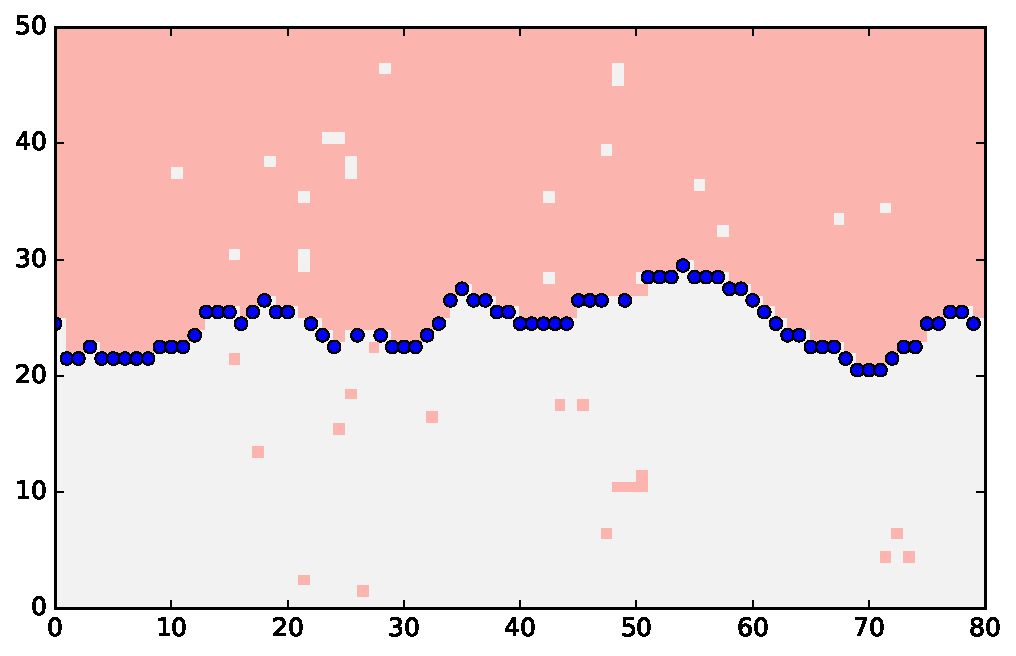
\includegraphics[width=\linewidth]{isingtosos/snap07.pdf}
	\end{minipage}%
	\begin{minipage}[t]{0.33\linewidth}
		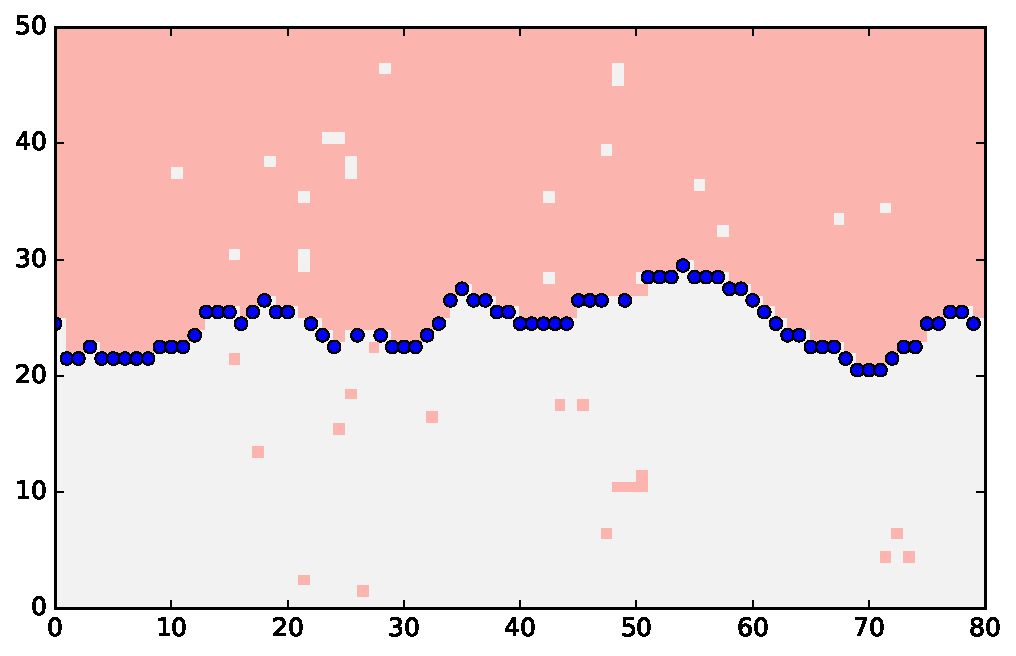
\includegraphics[width=\linewidth]{isingtosos/snap07.pdf}
	\end{minipage}
	\begin{minipage}[t]{0.33\linewidth}
		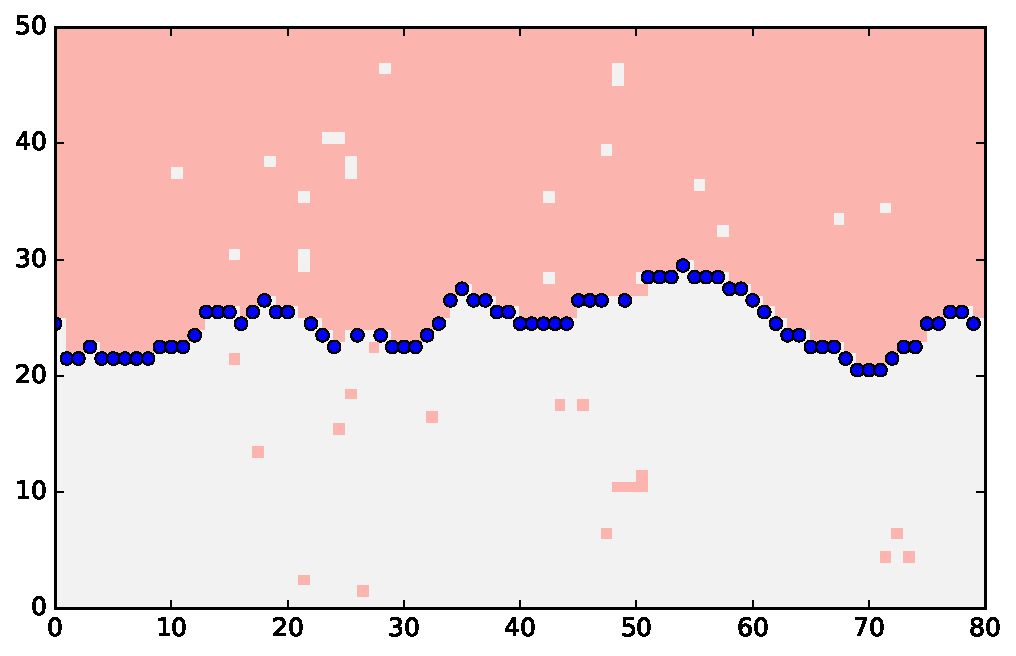
\includegraphics[width=\linewidth]{isingtosos/snap07.pdf}
	\end{minipage}
	\caption{Photo Ising périodique en X et Y, quenchin avec le temps }
	\label{amas-quench}
\end{figure}

\begin{figure}
	\begin{minipage}[t]{0.5\linewidth}
		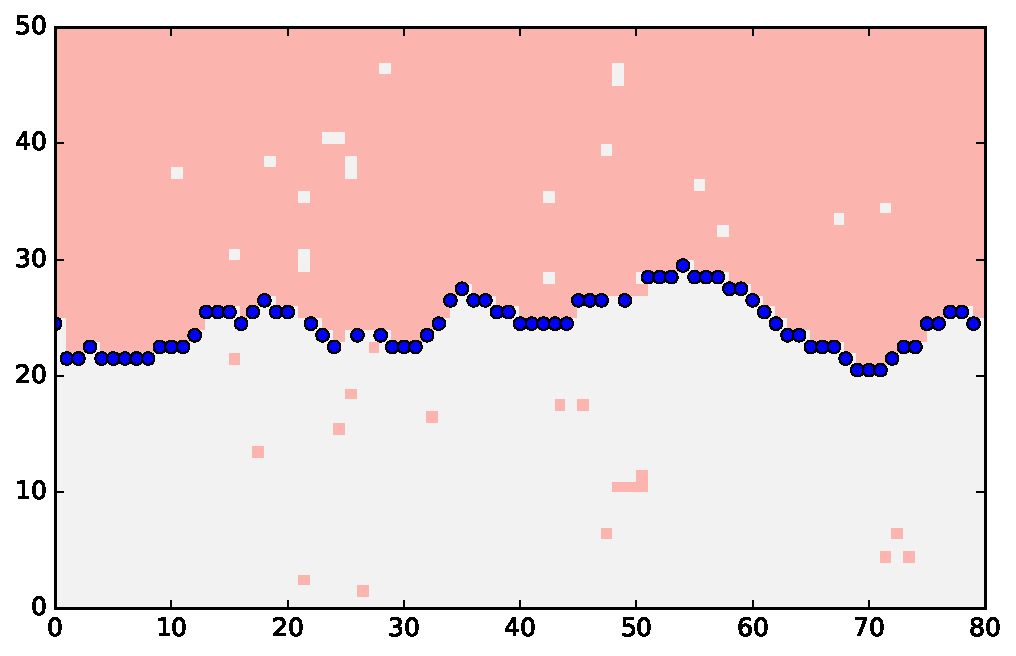
\includegraphics[width=\linewidth]{isingtosos/snap07.pdf}
	\end{minipage}%
	\begin{minipage}[t]{0.5\linewidth}
		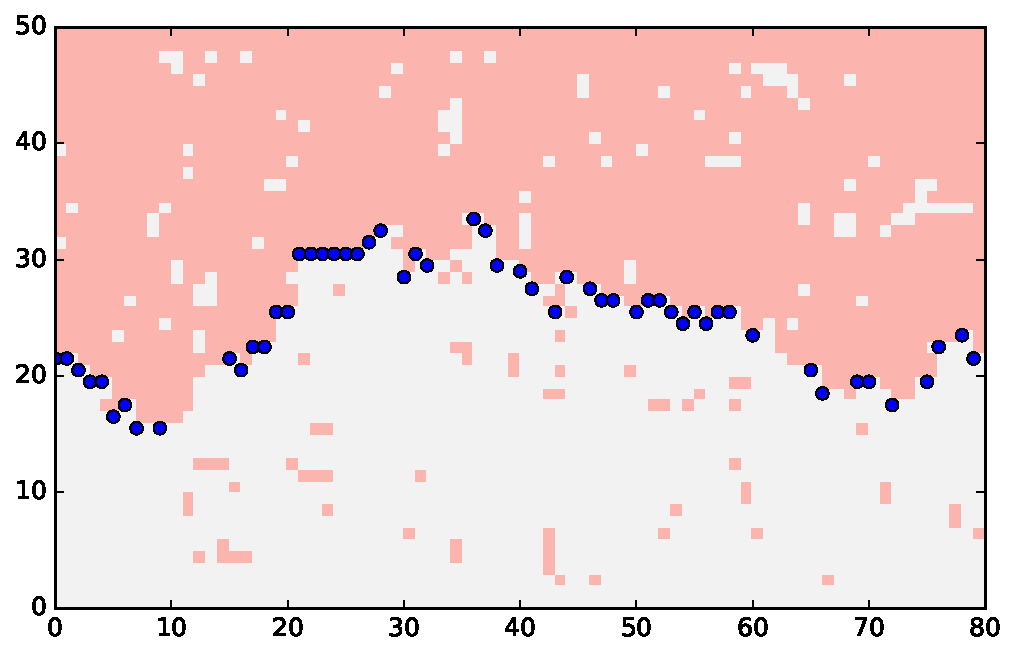
\includegraphics[width=\linewidth]{isingtosos/snap09.pdf}
	\end{minipage}
	\caption{Photo d'un modèle d'Ising à deux températures différentes($T=0.7 T_C$ et $T=0.95 T_C$ ) avec des conditions périodiques aux bords en X et fixés en Y qui forcent la présence d'une interface entre les phases $+$ (rose) et $-$ (blanc) du système. Plus la température est élevée et plus l'interface fluctue, jusqu'à cesser d'exister pour $T > T_C$. }
	\label{amas-fixe}
\end{figure}

  \section{Le modèle d'Ising}
  
  	Le modèle d'Ising fait partie de la catégorie des modèles sur réseau où l'interaction entre les particules du système se fait uniquement entre les plus proches voisins. Chaque particule au site $i$ possède deux états différents que l'on note $\sigma_i = \pm 1$, analogues aux spins en mécanique quantique. L'Hamiltonien d'un tel modèle s'écrit alors
\begin{equation}
	\mH =  - \sum_{\langle i j >} J_{ij} \sigma_i \sigma_j + \frac{V(\sigma_i)+V(\sigma_j)}{2}
\end{equation}
où $\langle ij >$ dénotent deux premiers voisins, $J_{ij}$ l'énergie d'interaction entre deux sites et $V(\sigma_i)$ le potentiel au site $i$.
En général, le modèle d'Ising est utilisé avec une énergie d'interaction constante entre tous les spins, soit $J_{ij} = J$. Les systèmes les plus connus possédant une énergie d'interaction non-constante sont  \textbf{trouver quelques exemples}.

En faisant la transformation\cite{ref23David} $n_i =  \frac{\sigma_i +1}{2}$ afin que $n_i(\sigma_i = 1) = 1$ et $n_i(\sigma_i = -1) = 0$, on obtient l'hamiltonient
\begin{equation}
	\mH =  - \sum_{\langle i j >}  J_{ij} \left( 4 n_i n_j -2 ( n_i+n_j) + 1 \right)+ \sum_{\langle i j >}  J_{ij} \frac{V(\sigma_i)+V(\sigma_j)}{2}  
\end{equation}
où le terme constant $\sum_{\langle i j >}  J_{ij}$ ne modifie la fonction de partition $\mZ$ que d'une constante peu importante pour les propriétés à l'équilibre du système. On définit alors 
\begin{equation}
	\mH_{LG} =  - 4 \sum_{\langle i j >}  J_{ij}  n_i n_j  + 2 \sum_{\langle i j >}  J_{ij}  (n_i+n_j) + \sum_{\langle i j >}  J_{ij} \frac{V(\sigma_i)+V(\sigma_j)}{2}  
\end{equation}
Le deuxième terme s'identifie à la présence d'un potentiel chimique pour les particules liquide-gaz. Une phase magnétique positive dans le modèle d'Ising s'apparente dès lors à un état de haute densité (un liquide), tandis qu'une phase négative est considérée comme une phase de basse densité, c'est-à-dire un gaz.
Ce modèle représente également un mélange binaire\cite{} entre deux types de particules $A$ et $B$ comme par exemple un polymère dans un solvant, les particules identiques s'attirant tandis que les particules d'un type différent se repoussent. 

En général, dans tous les modèles d'Ising étudiés, $J_{ij}$ est constante et égale à $J$. Nous prendrons cette approximation à partir de maintenant.

En absence de potentiel, le système est statistiquement découpé en amas (\textit{bulk}) de spins du même signe\ref{amas-quench}. La longueur de corrélation   $\mC= \mC(T,J)$ dépend fortement de la température et diverge près de la température critique. Une étude détaillée des grandeurs du modèle d'Ising proche du point critique\cite{onsager,3d} peut être retrouvée dans \cite{these_david}.

L'étude de l'interface entre les phases $+$ et $-$ nécessite la brisure de la symétrie de translation au sein du système. Cela peut se faire facilement soit par des conditions aux bords non-périodiques dans une direction, soit  par la présence d'un champ magnétique non-uniforme du style $V(y) = h |\frac{L_Y}{2}-y|$. 
Dans le cas de conditions aux bords fixes avec par exemple les spins de la rangée $0$ étant positifs et ceux de la rangée $L_Y$ négatifs, des clusters vont se former et créer une interface au milieu. Il est possible de favoriser une phase par rapport à l'autre grâce à un potentiel chimique (ou champ magnétique) $V(h_i) = -h \sigma_i$ \cite{}. Ce genre de modèle s'assimile à un système d'absorption d'un gaz sur réseau\cite{} ou de la croissance d'un matériau sur un substrat\cite{}

Le choix d'un champ magnétique du style $V(y) = - B |\frac{L_Y}{2}-y|$ modélise quant à lui l'effet d'un champ  sur un liquide binaire selon les expériences de Delville\cite{}. La présence d'un laser dans certaines régions du système peut modifier localement le potentiel chimique des particules, favorisant la présence d'un type par rapport à l'autre. L'épinglage\cite{} (\textit{pinning}) de l'interface auprès de la ligne de démarcation permet de l'étudier loin des bords du système.

	\section{Modèle Solid-On-Solid}
		
Quelle que soit la méthode utilisée, le système se simplifie dès lors que nous désirons étudier uniquement l'interface d'un système et non son ensemble, telles que les longueurs de corrélations dans le \textit{bulk}, l'aimantation moyenne, la chaleur spécifique ou la susceptilibté magnétique. À très basse température, les interfaces sont bien délimitées et il y a très peu de gouttes d'évaporations d'une phase dans l'autre. En considérant le système très peu mélangé, il est possible de définir la présence d'une phase par rapport à la hauteur $h_i$ de l'interface. Chaque spin prend la valeur
\begin{equation*}
	\sigma_{i,j} = \sgn(h_i-j)
\end{equation*}
où la fonction $\sgn(x)$ est égale à $+1$ si $x>=0$ et à $-1$ sinon. Cela revient à considérer que l'énergie d'interaction perpendiculaire est prohibitif par rapport aux liaisons parallèles à l'interface $J_\perp \gg J_\parallel$. 

\begin{figure}
	\centering
	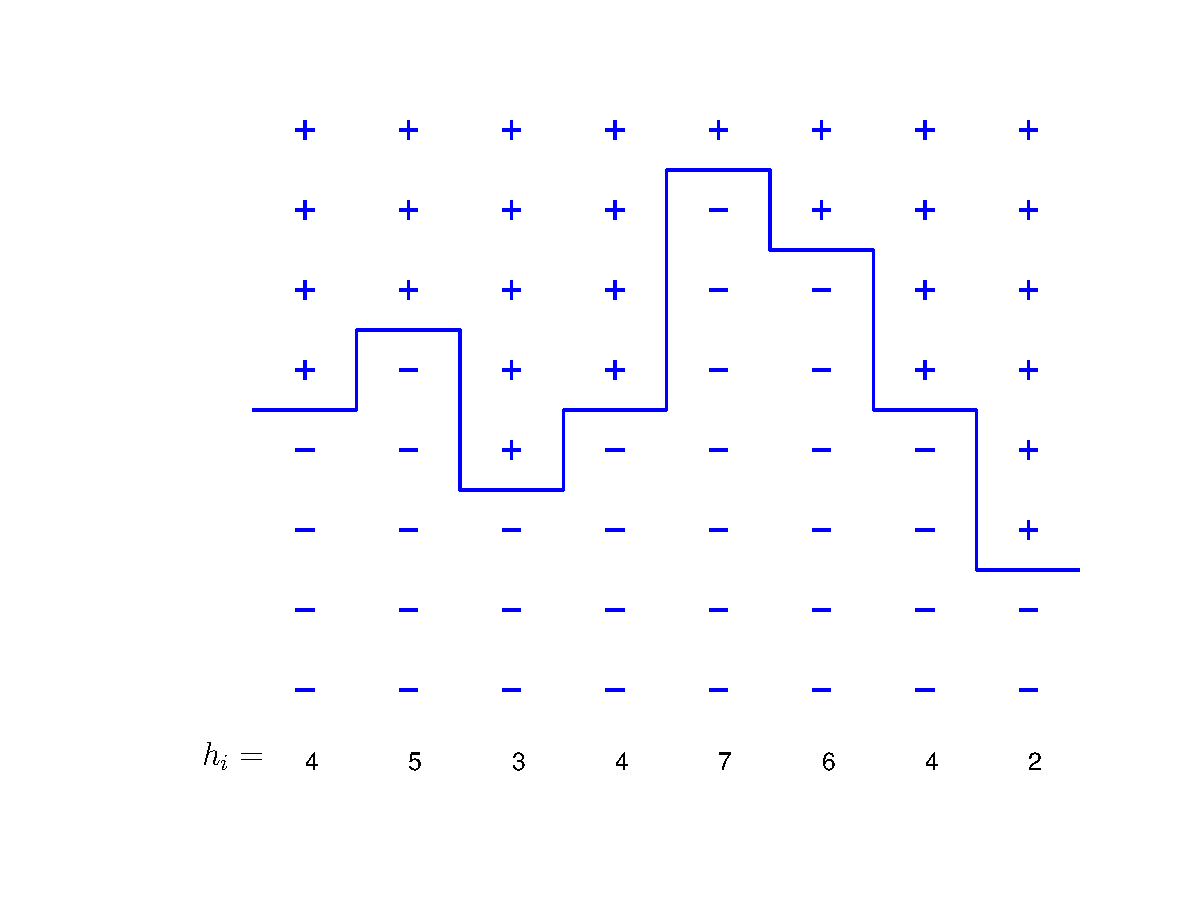
\includegraphics[width=0.7\linewidth]{isingtosos/figure-sos.pdf}
	\caption{Une configuration possible de modèle SOS. Dans la i-ème colonne le bord horizontal de l'interface passe à la hauteur $h_i$}
\end{figure}

En utilisant l'identité $\min(a,b)-\max(a,b)=|a-b|$, on a
\begin{align*}
    \sum_{j=0}^L \sgn(h-j)\sgn(h'-j) = L - 2 |h-h'|
\end{align*}
Ainsi, pour un système de longueur $L_X$ et de largeur $L_Y$ l'hamiltonien du modèle d'Ising en absence de potentiel se réécrit comme 
\begin{align*}
    H &= - J \sum_{<ij>} \sigma_i \sigma_j  \nn
    &= -J \sum_{i,j} \sigma_{i,i} ( \sigma_{i+1,j}+\sigma_{i-1,j}+\sigma_{i,j+1}+\sigma_{i,j-1} ) \nn
    &= -J \sum_{i,j} \sgn(h_i-j) ( \sgn(h_{i+1}-j)+\sgn(h_{i-1}-j)+\sgn(h_{i}-j-1)+\sgn(h_{i}-j+1) ) \nn
    &= 4 J L_X (2-L_Y) +4J \sum_i |h_i-h_{i+1}|
\end{align*}
Le terme $|h_i-h_{i+1}|$ représente la surface de contact horizontale entre les deux phases qui dépend directement de la hauteur, tandis que le terme constant représente la surface de contact verticale.
En retirant la partie constante de l'énergie et simplifiant $4 J = J$ et en gardant $L_X = L$, nous obtenons l'hamiltonien du \textbf{modèle Solid-On-Solid}
\begin{equation}
    H = J \sum_i |h_i-h_{i+1}|
    \label{hamil-sos}
\end{equation}

On calcule les observables du système de manière analogue. 

\begin{itemize}
	\item La magnétisation moyenne par site $M = <\sigma_{ij}>$ devient $M = <h_i> = \frac{1}{L}\sum_i h_i$
	\item La magnétisation moyenne à $j$ donné est $m(j) = \frac{1}{L} \sum_i \sgn(h_i-j)$
	\item L'énergie moyenne par site $E = \frac{1}{L}  \sum_i |h_i-h_{i+1}|$
\end{itemize}

Nous avons ici réussi à réduire la dimensionalité du système en ne prenant en compte que la hauteur $h_i$ au site $i$. L'énergie du système est alors décrite par la différence de hauteur entre deux sites voisins, et $\beta J$ prend ici alors le rôle de la tension de surface.

Puisqu'il n'y a plus de transition de phase possible dans ce modèle, la température critique $\beta_C$ du modèle d'Ising n'a plus de rôle à jouer ici. Pour rester dans le domaine de l'approximation, si nous désirons comparer les résultats avec ceux du modèle d'Ising, il faudra veiller à rester dans le domaine $T<T_C$, l'approximation étant de plus en plus valable plus la température est basse. Par la suite, puisque nous désironts étudier le modèle SOS et non le comparer avec le modèle d'Ising, nous prendrons, sauf cas contraire explicité, $\beta = \beta_C$ et $J=1$ par soucis de simplicité. 

  \subsection{Matrice de Transfert}

	De manière plus générale, l'Hamiltonien d'un système avec des interactions entre les particules peut se réécrire comme $H = \sum_{\langle ij >} H(i,j)$ avec
\begin{equation*}
  H(h_i,h_{i+1}) = f(h_i,h_{i+1}) + V(h_i,h_{i+1}) 
\end{equation*}
où $f(h_i,h_j)$ est l'énergie d'interaction entre plus proches voisins et $V(h_i,h_j)=\frac{V(h_i)+V(h_j)}{2}$ le potentiel symmétrisé.
La fonction de partition de notre système s'écrit alors 

\begin{equation*}
 Z = \sum_{h_1 h_2 ... h_L} e^{- \beta \sum_{i} H(h_i,h_{i+1})}  
   = \sum_{h_1 h_2 ... h_L} \prod_{i} e^{-\beta H(h_i,h_{i+1})} 
\end{equation*}
La matrice $T(i,j) = e{-\beta H(i,j)}$ est appelée matrice de transfert. Cette matrice est périodique aux bords, c'est-à-dire $T(L,L+1) = T(L,1)$ et est symétrique, ce qui implique qu'elle est diagonalisable dans la base des vecteurs propres $|\lambda >$ de valeur propre $\lambda$. On dénote par $\lambda_0$ la plus grande valeur propre de $T$, -par $\lambda_1$ la deuxième plus grande valeur propre et ainsi de suite.
Ainsi la fonction de partition devient\cite{}
\begin{equation}
  Z = \sum_{\sigma_1 \sigma_2 ... \sigma_{L}} \prod_{i} T(i,i+i) = Tr T^L  = \sum_\lambda \langle\lambda | T^L | \lambda> = \sum_\lambda \lambda^L
\end{equation}

Dans la limite thermodynamique $L \to \infty$, seuls les plus grands vecteurs propres jouent un rôle. Afin de calculer les observables de notre système, il convient d'introduire la matrice des hauteurs $\tilde{M}(i,j) = \delta_{ij} i$. Nous avons donc \footnote{Pour une démonstration plus détaillée sur les matrices de transfert, se référer à \cite{matrice_transfert}}
\begin{itemize}
	\item L'énergie libre :  
	\begin{equation}
		F =  - \frac{1}{L \beta} \ln(Z) \simeq - \frac{1}{\beta } \ln( \lambda_0)
	\end{equation}
	\item La densité de probabilité qu'un site se trouve à la hauteur $h$ : 
	\begin{equation}
		p(h) = \frac{1}{Z} \sum_\lambda \lambda^L \langle\lambda | h >^2 \simeq \langle \lambda_0 | h >^2
	\end{equation}
	\item La magnétisation moyenne :
	\begin{equation}
		M = \langle h > = \langle \lambda_0 | \tilde{M} | \lambda_0 > 
	\end{equation}
	\item La variance des hauteurs :
	\begin{equation}
		\sigma = \langle (h - \langle h >)^2 > =  \langle \lambda_0 | \tilde{M}^2 | \lambda_0 >
	\end{equation}
\end{itemize}

	\subsection{Stabilité de l'interface}

	Soit $\phi_\lambda(h)$ la projection du vecteur propre associé à la valeur propre $\lambda$ de la matrice de transfert sur la base des hauteurs dans un système infini de par et d'autre de l'interface. En absence de potentiel\cite{guyer1979}, l'équation du vecteur propre donne
\begin{align}
	\sum_{h=-\infty}^\infty T(h,h') \phi_\lambda(h) = \lambda \phi_\lambda(h')
\end{align}
En introduisant l'ersatz $\phi_\lambda(h) = \alpha^h$ qui respecte la symétrie du système, et en séparant de la somme les termes pour $h$ négatifs et positifs, on trouve aisément que 
\begin{align}
	\frac{\sinh(\beta J)}{\cosh(\beta J)-(\alpha+\frac{1}{\alpha})} \alpha^{h'} = \alpha^{h'} \lambda
\end{align}
Dans la limite thermodynamique, la probabilité de présence de l'interface à la hauteur $h$ est $p(h) = <\lambda_0|h>^2 = |\phi_0(h)|^2$. Le système ne possédant aucune brisure de symétrie particulière, la probabilité $p(h)$ se doit d'être bornée pour tout $h$. Dès lors, l'ersatz supposé $\phi_\lambda(h) = \alpha^h$ implique que $\alpha$ soit de la forme $e^{ik}$ où $k$ est la longueur d'onde associée à la valeur propre $\lambda$. On obtient que 
\begin{align}
	\phi_k(h) =& e^{ikh} \\
	\lambda_k =& \frac{\sinh(\beta J)}{\cosh(\beta J) - \cos(k)}
\end{align}


Dans le cas plus général où l'hamiltonien s'écrit de la forme $T(h,h') = f(|h-h'|)$, on trouve 
\begin{align}
	\lambda_k = \sum_{h=0}^\infty f(h)(\alpha^h+\alpha^{-h}) - f(0)
\end{align}

L'existence d'une solution de ce genre indique que l'interface n'est pas localisée dans le cas d'un système infini (ou semi-infini) en absence de tout potentiel, ce qui conduit à de nombreux problèmes numériques. 

Il est à noter qu'à $\beta=0$, c'est-à-dire pour une température infinie, la matrice de transfert est uniformément égale à $1$, menant à des vecteurs propres nuls. Dans cette limite, l'interface n'existe plus, le modèle SOS n'est donc pas valable. De même, pour une température nulle $\beta=\infty$, la matrice de transfert devient la matrice identité. Les valeurs propres deviennent toutes égales à $1$ et les vecteurs propres sont $\phi_i(h) = \delta_{h,i}$ où ici $i$ est l'indice de la i-ème valeur propre $\lambda_i = 1$. La probabilité de trouver l'interface à la hauteur $h$ devient $p(h) = \frac{1}{Z}\sum_{i} <\lambda_i | h >^2 = 1$. La température nulle a pour effet de geler l'interface sur une seule hauteur, mais toutes les hauteurs sont équiprobables. Bien que les micro-états soient extrêmement différents que pour une température finie, les propriétés macroscopiques sont identiques à cause du même poids statistique associé à chaque état.


Historiquement, une manière facile de localiser l'interface est de rajouter un potentiel $V(h) = -B \delta_{h,0}$ \cite{chui}. La présence du potentiel n'affecte pas la parité du système mais peut introduire un surplus de particules en $0$. La recherche d'un état lié nous donne un ersatz de la forme 
\begin{align}
	\phi_\lambda(h) = \begin{cases} |\alpha|^h & \text{si } h \neq 0 \\ \phi_{\lambda,0} & \text{sinon} \end{cases} 
\end{align}
L'équation du vecteur propre devient
\begin{align}
	\sum_{h=-\infty}^\infty e^{\beta |h-h'|- \beta B \delta_{h,0}} \phi_\lambda(h) = \lambda \phi_\lambda(h')
\end{align}
En notant $T(h,h') = R^{|h-h'|}$ pour $h \neq h' \neq 0$,  on obtient la même équation à un signe près dans l'exposant que l'on soit à $h'>0$ ou $h'>0$
\begin{align}
	\left( \frac{R}{\alpha} \right)^{\pm h'} \left[ \phi_{\lambda,0} + \frac{R \alpha}{1 - R \alpha} + \frac{\alpha}{R - \alpha} \right] + \left[ \frac{1}{1-R \alpha} - \frac{R}{R-\alpha} \right] = \lambda
\end{align}
Puisque cette équation est vraie pour tout $h'$, le premier terme doit être nul, ce qui nous donne
\begin{align}
	\phi_{\lambda,0} &= - \frac{\alpha}{R-\alpha}-\frac{R \alpha}{1-R \alpha} \\
	\lambda &= \frac{1}{1-R \alpha} - \frac{R}{R-\alpha}
\end{align}
L'équation du vecteur propre à $h'=0$ nous donne par ailleurs 
\begin{align}
	\phi_{\lambda,0} + 2 \frac{R \alpha}{1-R \alpha} = \lambda \phi_{\lambda,0} e^{-\beta B}
\end{align}
L'existence d'une solution cohérente $\alpha < 1$ autorise la présence d'une interface localisée grâce au pinning.

D'autres méthodes existent pour confiner l'interface. Le cisaillement d'une interface diminue sa largeur et permet de la localiser dans l'espace. On peut également proposer deux potentiels chimiques différents pour chaque phase à une hauteur de l'interface prédéfinie, comme le ferait un laser dans les expériences de cisaillement\cite{delville} dans un système semi-infini. Cet cas sera étudié plus loin. Dans un système infini, une autre possibilité est de définir un champ magnétique symétrique rendant plus difficile la présence de l'interface loin de $0$. Nous utiliserons ici un potentiel du style
\begin{align}
		  V(h) = B |h|
\end{align}

Il est facile de se convaincre que loin de $0$ le coût énergétique est si grand que la probabilité que l'interface s'y trouve soit petite, impliquant que l'interface est localisée. La position moyenne de l'interface se situe au minimum du potentiel qui est dans ce cas $0$. 

	\subsection{Modèle Particle-Over-Particle }
	
	Le modèle Solid-On-Solid est l'approximation standard du modèle d'Ising car elle est étudiable analytiquement via sa matrice de transfert. 	Tout comme lorsque l'on déforme un flan seules les particules à l'interface flan-air peuvent bouger, dans le modèle SOS les particules loin de l'interface entre les deux phases ne peuvent bouger via l'agitation thermique. 
	Nous proposons alors un modèle un peu plus physique, dans lequel chaque particule a le droit de bouger. Au lieu de ne considérer que la hauteur $h_i$ au site $i$, nous considérons qu'il existe $h_i$ particules empilées les unes sur les autres. Lors d'un déplacement, nous prenons une particule au hasard pour la déplacer vers le haut de la pile, puis vers un autre site $j$. 
	Ainsi la fonction de partition devient
	
\begin{equation}
	Z = \sum_{h_1 h_2 ... h_L} e^{- \beta \sum_{i} H(i,i+1)} \frac{N!}{\prod_i n_i!} = N! \sum_{h_1 h_2 ... h_L} e^{- \beta \sum_{i} H(i,i+1) -\sum_i \ln(n_i!)}
\end{equation}

La matrice de transfert symétrisée devient donc
\begin{equation}
	T(h,h') = e^{-J |h-h'| - \frac{1}{2}(\ln(h!)-\ln(h'!)}
\end{equation}
où les termes $\ln(h)$ proviennent de l'entropie générée par la présence des particules au sein même des sites. À notre connaissance, ce modèle n'a pas été aussi étudié que le modèle SOS bien qu'il soit physiquement plus proche du modèle d'Ising initial. Le fait que la matrice de transfert ne soit pas résolvable analytiquement en est peut-être la cause. 



























\begin{comment}
		\section{SOS Hamiltonian}
		%%%%%%%%%%%%
		
		In the following, we present three Solid-On-Solid models with different magnetic fields. 
		The SOS interaction between nearest neighboors is of the form $f(i,j) = |h_i - h_j|$. 
		This kind of interaction prevents big fluctuations between two nearest neighboors and is directly related to the Ising model in the approximation where there are no overhangs between the two phases. \textcolor{blue}{see my notes for the derivation}
		
		In the absence of a magnetic field, the interface will fluctuate around its center. Shown below an typical SOS interface for an $L_X=50$ and a $L_Y=60$ after $10^5$ Monte Carlo steps.
		
		%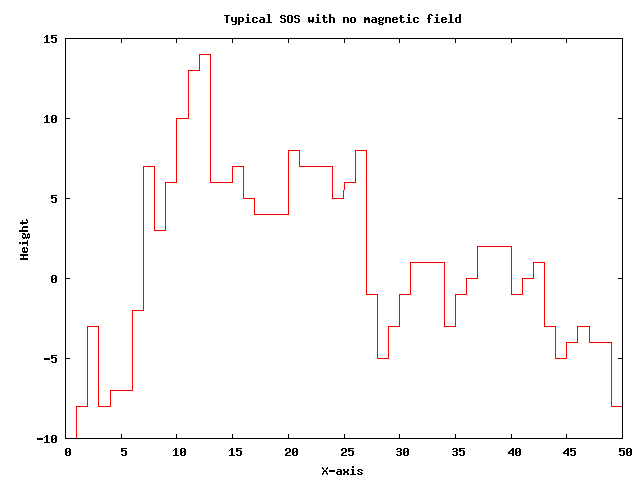
\includegraphics[width=10cm]{nomag.png}
		
		
		%%%%%%
		\subsection{Model $g(i) = h_i$ (model A)}
		%%%%%%
		
		This model replicates the effect of a homogeneous magnetic field. The bigger the magnetic field $B$ (which can be positive or negative), the further the interface is driven with a symetry breaking. 
		
		\begin{align}
		  H(i,j) = J |h_i-h_j| + B \frac{h_i + h_j}{2}
		\end{align}
		
		%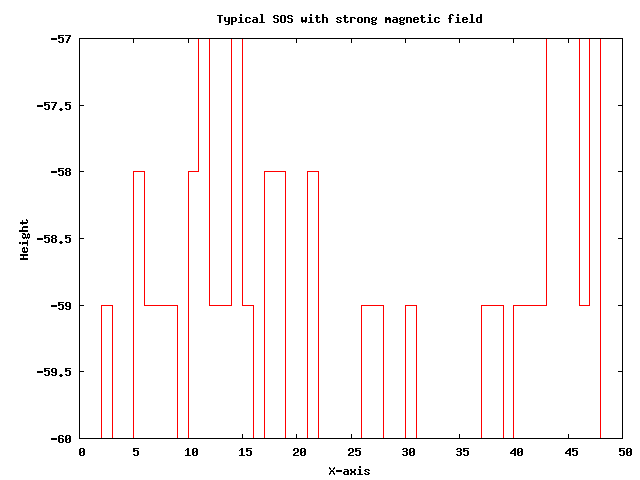
\includegraphics[width=10cm]{normal.png}
		
		For an infinite magnetic field, we clearly see that the interface gets flattened over on of the edge. The resulting single state avalaible in this limit is the flat interface, with all sites beeing over or under it, depending on the sign of $B$.
		
		In the limit $B \rightarrow \infty$, the interface will flatten to the bottom edge, resulting in a single state of energy 
		\begin{align}
		  F(B \rightarrow \infty) = - B L_Y
		\end{align}
		
		The free energy for at $B=0$ is thus given by equation \ref{free_energy} as
		\begin{align}
		  F(0) = B L_X L_Y - \int_0^\infty m(B)dB
		  \label{energymodela}
		\end{align}
		with $m(B) = \langle\sum_i h_i> = L_Y$
		
		%%%%%%
		\subsection{Model $g(i) = |h_i|$ (model B)}
		%%%%%%
		
		This model uses a stagged magnetic field analoguous to the action of a laser on a binary mixture. The further we get from the mean position, the higher is the energy. In order to minimize the energy, the system will have a tendency to be pinned, leading to a very flat interface. 
		
		\begin{align}
		  H(i,j) = J |h_i-h_j| - B \frac{|h_i| + |h_j|}{2}
		\end{align}
		
		%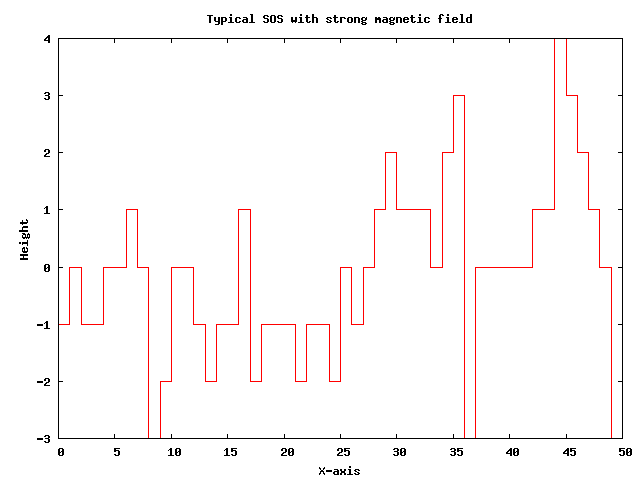
\includegraphics[width=10cm]{stagged.png}
		
		In the limit $B \rightarrow \infty$, the free energy $F$ will be equal to $0$, while the magnetisation $m(B \rightarrow \infty) = \langle\sum_i |h_i|> = 0$ also.
		
		%%%%%%
		\subsection{Model $g(i) = -|h_i|$ (model C)}
		%%%%%%
		
		This model is the same as the previous one, except with a switch of sign. In this case, the magnetic field will have a depinning effect leading to a scattering of the heights around both edges. \textcolor{red}{I don't really get yet the argument about the competition between entropy and energy.}
		
		\begin{align}
		  H(i,j) = J |h_i-h_j| - B \frac{|h_i| + |h_j|}{2}
		\end{align}
		
		%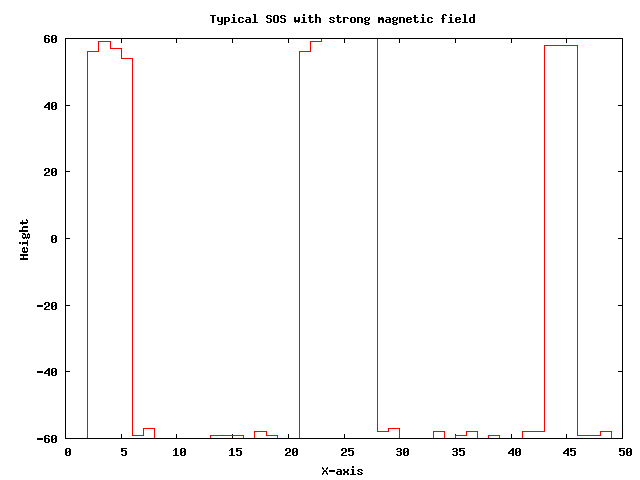
\includegraphics[width=10cm]{negstagged.png}
		
		In the $B \rightarrow \infty$ limit, we have then a scattered system. How can we compute its free energy ? Sites will be at $h_i=\pm L_Y$ , leading to an easy $2\times 2$ transfer matrix.
		\begin{align}
		  Z = e^{\beta B L_Y L_X} Tr( (e^{-\beta J \frac{L_Y}{2} \sum_i |\sigma_i - \sigma_j| })^{L_X} )
		\end{align}
		where $\sigma_i = \pm 1$
		
		The transfer matrix is then given as
		
		\begin{align}
		T= e^{\beta B L_Y}
		  \begin{pmatrix}
		    1 & e^{-\beta 2 J L_Y} \\
		    e^{-\beta 2 J L_Y} & 1
		  \end{pmatrix}
		\end{align}
		Its eigenvalues are $\lambda_\pm = e^{\beta B L_Y}( 1 \pm e^{-\beta 2 J L_Y})$, giving a partion function 
		\begin{align}
		  Z = e^{\beta B L_Y L_X} \times ((1 - e^{-\beta 2 J L_Y})^{L_X} + (1 + e^{-\beta 2 J L_Y})^{L_X} )
		\end{align}
		
		The free energy from \ref{deffree_energy} is 
		\begin{align}
		  F(B\rightarrow \infty) = - L_Y B - \frac{1}{\beta} \ln \left( 1 + e^{-\beta 2 J L_Y} \right)
		  \label{energymodelc}
		\end{align}
		which, in the limit of $L_X \rightarrow \infty$ converges to \ref{energymodela}. This is easily explained as the energy to switch from a side to another increases so much that at some point the interface will be pinned to one of the edges, resulting in the same single state.
		
		\begin{figure}
		%  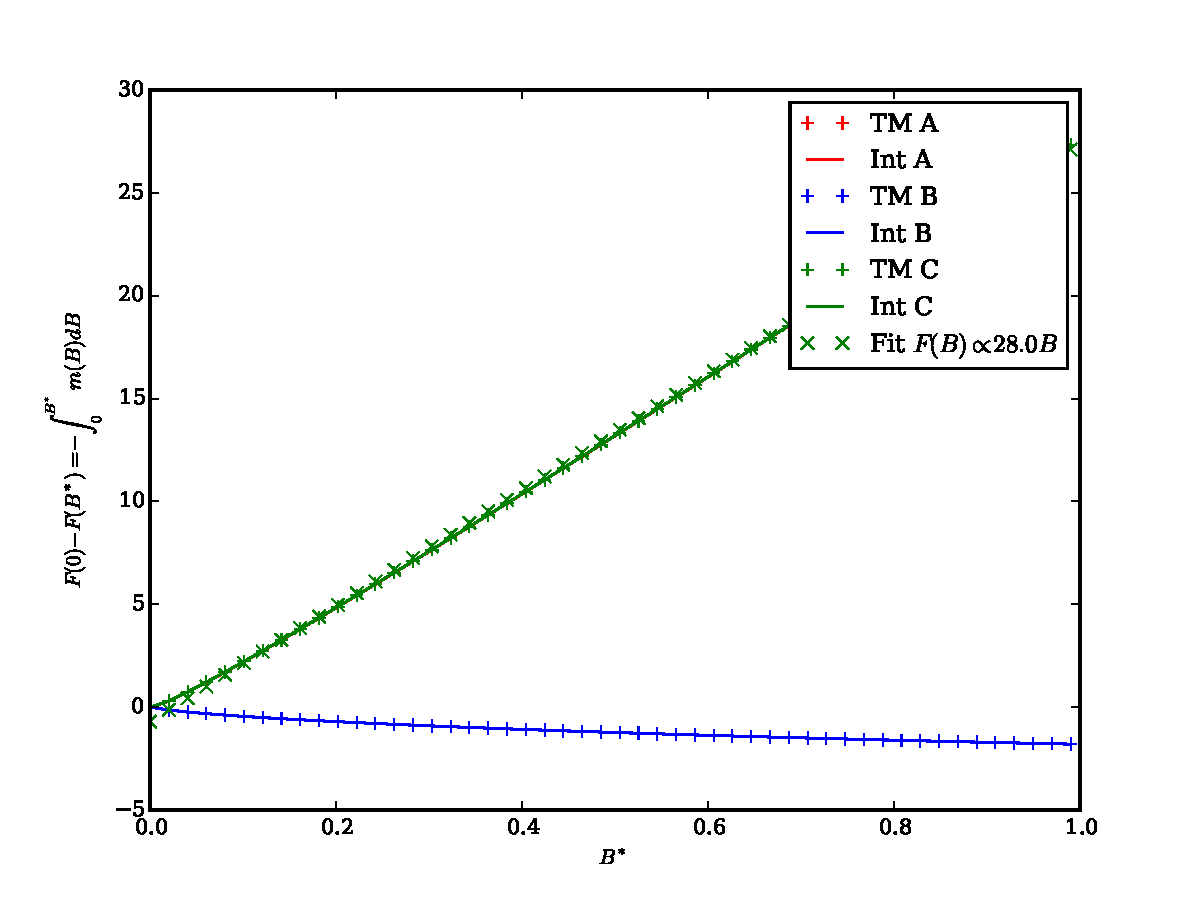
\includegraphics[width=13cm]{comparison.pdf}
		  \caption{Computation of both terms in \ref{free_energy} in the limit $L_X \rightarrow \infty$ and $L_Y=30$ for the three different models. We see that models A and C have a very similar behaviour even for very small $B$. The linear fit does indeed give a relation $F(0) - F(B) = L_Y \times B$}
		\end{figure}
		
		%%%%%%%%%%%%
		\newpage
		\section{Numerical results}
		%%%%%%%%%%%%
		
		The diffusion of particles in a system can be mapped in an Ising model pretty easily if we assume the conservation of particles through time in our Monte Carlo dynamics. That means that $\sum h_i = K$, with $K$ a constant defined by the initial conditions. This condition can be enforced in the partition function if we only take the microstates satisfying our constraint. Sadly, this constraint is about the microstates and can not be transposed into our Hamiltonian, making the Transfer Matrix useless for such a case. 
		
		The question we want to adress is thus : how big is the difference between the constrained and the unconstrained dynamic in the computation of the free energy ? Is the limit $B^{\ast} \rightarrow \infty$ the same for the three models for both dynamics ? 
		Figure \ref{compGlau} conforts us in the conformity between the Glauber dynamic and the Transfer Matrix method. 
		
		\begin{figure}[h]
		%  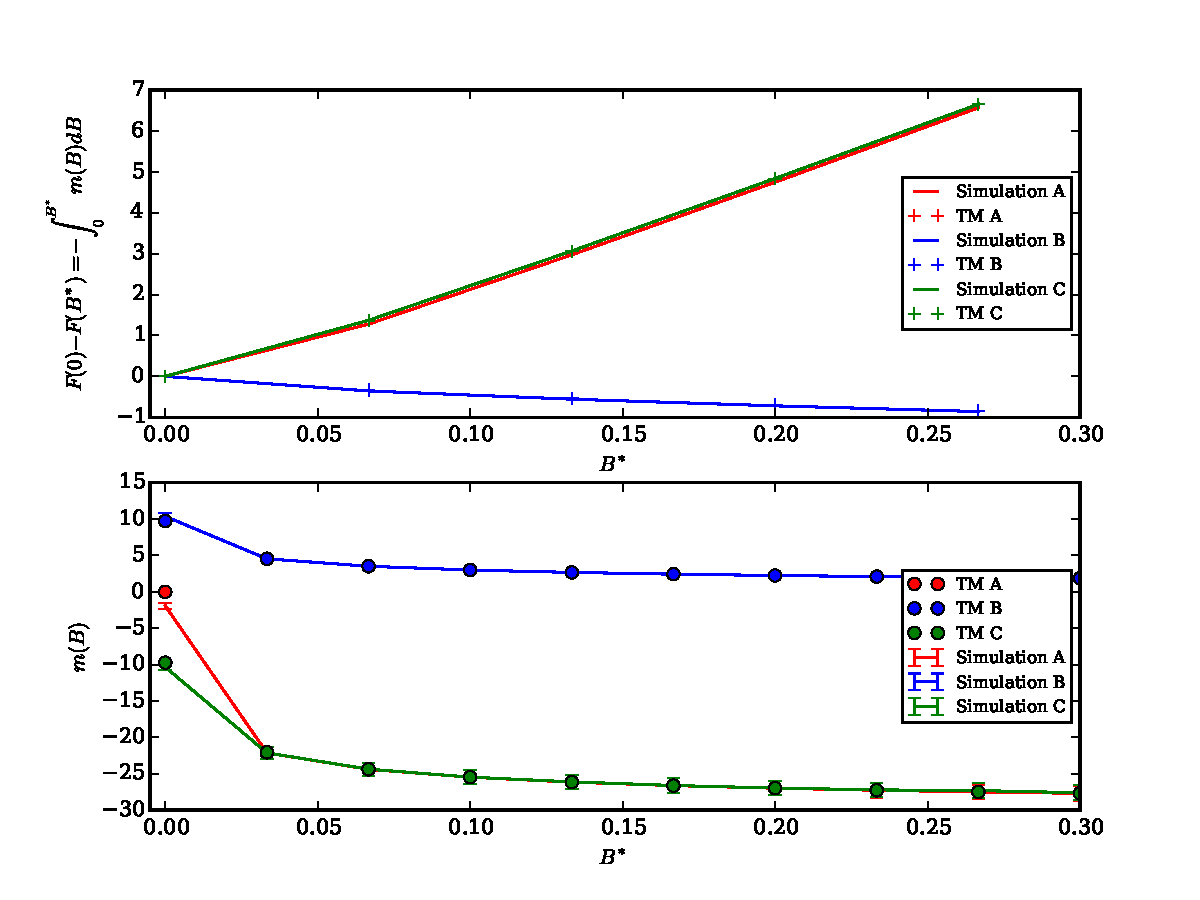
\includegraphics[width=13cm]{ModGlau.pdf}
		  \caption{Computation of the free energy (above) and the magnetisation (below) for the three models in a Glauber dynamics (unconstrained dynamics) through simulations (with error bars) and exact transfer matrix diagonalization.}
		  \label{compGlau}
		\end{figure}
		
		When comparing to the Kawasaki dynamic in Figure \ref{compKaw}, we start seeing some differences. First, in model A the magnetization of our system is always  equal to $0$, by construction of our Kawasaki dynamics, meaning that the computation of the free energy is a tricky one. Luckily, Model A is very similar to Model C with respect to the posible microstates, except some walls that do not add a significan free energy into the system. This means that the results we obtain in Model C are roughly the same as in Model A ! This allows us to drop Model A from the discussion from now on and get retrieve its general behaviour and properties from Model C.
		
		As expected, the constrained dynamics adds some variance with respect to the Transfer Matrix. 
		
		\begin{figure}
		%  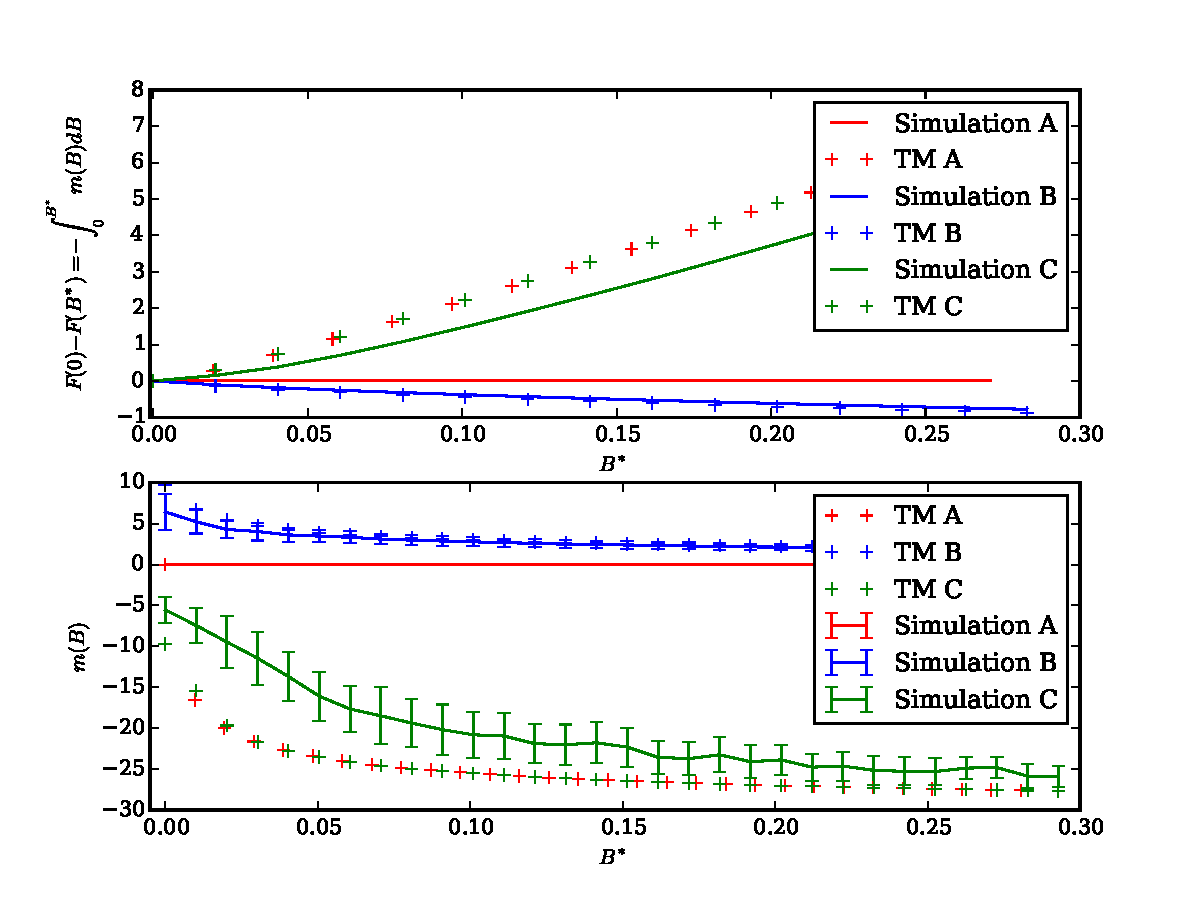
\includegraphics[width=13cm]{ModKaw.pdf}
		  \caption{Computation of the free energy (above) and the magnetisation (below) for the three models in a Kawasaki dynamics (constrained dynamics) through simulations (with error bars) and exact transfer matrix diagonalization. The error in magnetization of Model A is exactly equal to 0, by construction.}
		  \label{compKaw}  
		\end{figure}

  \section{Discretization of the system with respect to continuous models}
    \subsection{Correlation length and temperature}
\end{comment}






\begin{comment}

  \section{Le modèle d'Ising}



Le modèle d'Ising est un modèle extrêmement puissant pour modéliser diverses interactions complexes, que ce soit des gaz sur réseau ou des liquides binaires. Néanmoins, c'est cette même complexité qui nous oblige à avoir des simulations de Monte Carlo relativement longues et laborieuses, en dehors de toute possibilité d'analyse mathématique rigoureuse dans certaines conditions extrêmes qui sont celles qui nous intéressent ici. 

Lorsque nous nous intéressons aux effets de taille finie comme l'effet Casimir critique\cite{}, il est important que notre système puisse subir une transition de phase. Néanmoins, il existe des modèles bien plus faciles qui suffisent à expliquer une phénoménologie extrêmement analogue, celle de l'effet Casimir. Pour cet effet, il suffit d'avoir une interface entre deux phases et des conditions aux bords qui empêchent l'interface de fluctuer à sa guise. De cette frustration naît de manière effective une interaction entre les deux murs. Afin d'avoir quelques résultats analytiques, nous avons opté pour une approximation du modèle d'Ising qui ne retient que ce qui le plus important : l'interface.

\begin{figure}
    \centering
    \begin{subfigure}[b]{0.475\textwidth}
        \centering
        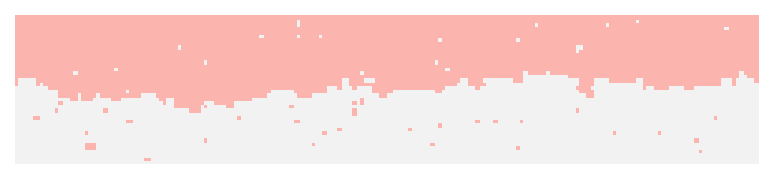
\includegraphics[width=\textwidth]{intro/t-70.pdf}
        \caption{$T=0.70 T_C$}
    \end{subfigure}
    \hfill
    \begin{subfigure}[b]{0.475\textwidth}  
        \centering 
        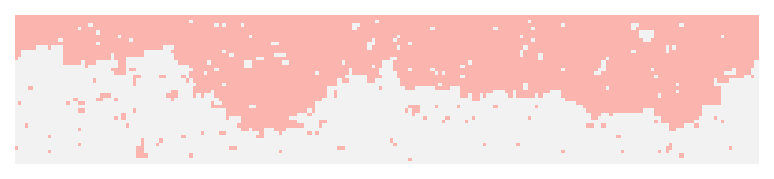
\includegraphics[width=\textwidth]{intro/t-85.pdf}
        \caption{$T=0.85 T_C$}        
    \end{subfigure}
    \vskip\baselineskip
    \begin{subfigure}[b]{0.475\textwidth}   
        \centering 
        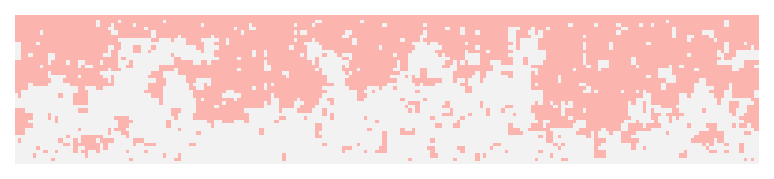
\includegraphics[width=\textwidth]{intro/t-100.pdf}
        \caption{$T= T_C$}        
    \end{subfigure}
    \quad
    \begin{subfigure}[b]{0.475\textwidth}   
    \centering 
        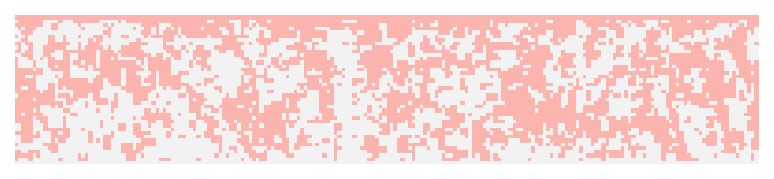
\includegraphics[width=\textwidth]{intro/t-130.pdf}
        \caption{$T=1.30 T_C$}        
    \end{subfigure}
	\caption{Photo d'un modèle d'Ising avec des conditions périodiques aux bords en X et fixés en Y qui forcent la présence d'une interface entre les phases $+$ (rose) et $-$ (blanc) du système. Plus la température est élevée et plus l'interface fluctue, jusqu'à cesser d'exister pour $T \greater T_C$. }
\end{figure}

  
  	Le modèle d'Ising fait partie de la catégorie des modèles sur réseau où l'interaction entre les particules du système se fait uniquement entre les plus proches voisins. Chaque particule au site $i$ possède deux états différents que l'on note $\sigma_i = \pm 1$, analogues aux spins en mécanique quantique. L'Hamiltonien d'un tel modèle s'écrit alors
\begin{equation}
	\mH =  - \sum_{\langle i j >} J_{ij} \sigma_i \sigma_j + \frac{V(\sigma_i)+V(\sigma_j)}{2}
\end{equation}
où $\langle ij >$ dénotent deux premiers voisins, $J_{ij}$ l'énergie d'interaction entre deux sites et $V(\sigma_i)$ le potentiel au site $i$.
En général, le modèle d'Ising est utilisé avec une énergie d'interaction constante entre tous les spins, soit $J_{ij} = J$. Les systèmes les plus connus possédant une énergie d'interaction non-constante sont  \textbf{trouver quelques exemples}.

En faisant la transformation\cite{ref23David} $n_i =  \frac{\sigma_i +1}{2}$ afin que $n_i(\sigma_i = 1) = 1$ et $n_i(\sigma_i = -1) = 0$, on obtient l'hamiltonient
\begin{equation}
	\mH =  - \sum_{\langle i j >}  J_{ij} \left( 4 n_i n_j -2 ( n_i+n_j) + 1 \right)+ \sum_{\langle i j >}   \frac{V(\sigma_i)+V(\sigma_j)}{2}  
\end{equation}
où le terme constant $\sum_{\langle i j >}  J_{ij}$ ne modifie la fonction de partition $\mZ$ que d'une constante peu importante pour les propriétés à l'équilibre du système. On définit alors 
\begin{equation}
	\mH_{LG} =  - 4 \sum_{\langle i j >}  J_{ij}  n_i n_j  + 2 \sum_{\langle i j >}  J_{ij}  (n_i+n_j) + \sum_{\langle i j >}  \frac{V(\sigma_i)+V(\sigma_j)}{2}  
\end{equation}
Le deuxième terme s'identifie à la présence d'un potentiel chimique pour les particules liquide-gaz. Une phase magnétique positive dans le modèle d'Ising s'apparente dès lors à un état de haute densité (un liquide), tandis qu'une phase négative est considérée comme une phase de basse densité, c'est-à-dire un gaz.
Ce modèle représente également un mélange binaire\cite{} entre deux types de particules $A$ et $B$ comme par exemple un polymère dans un solvant, les particules identiques s'attirant tandis que les particules d'un type différent se repoussent. 

En général, dans tous les modèles d'Ising étudiés, $J_{ij}$ est constante et égale à $J$. Nous prendrons cette approximation à partir de maintenant.

En absence de potentiel, le système est statistiquement découpé en amas (\textit{bulk}) de spins du même signe\ref{amas-quench}. La longueur de corrélation   $\mC= \mC(T,J)$ dépend fortement de la température et diverge près de la température critique. Une étude détaillée des grandeurs du modèle d'Ising proche du point critique\cite{onsager,3d} peut être retrouvée dans \cite{these_david}.

L'étude de l'interface entre les phases $+$ et $-$ nécessite la brisure de la symétrie de translation au sein du système. Cela peut se faire facilement soit par des conditions aux bords non-périodiques dans une direction, soit  par la présence d'un champ magnétique non-uniforme du style $V(y) = h |\frac{L_Y}{2}-y|$. 
Dans le cas de conditions aux bords fixes avec par exemple les spins de la rangée $0$ étant positifs et ceux de la rangée $L_Y$ négatifs, des clusters vont se former et créer une interface au milieu. Il est possible de favoriser une phase par rapport à l'autre grâce à un potentiel chimique (ou champ magnétique) $V(h_i) = -h \sigma_i$ \cite{}. Ce genre de modèle s'assimile à un système d'absorption d'un gaz sur réseau\cite{} ou de la croissance d'un matériau sur un substrat\cite{}

Le choix d'un champ magnétique du style $V(y) = - B |\frac{L_Y}{2}-y|$ modélise quant à lui l'effet d'un champ  sur un liquide binaire selon les expériences de Delville\cite{}. La présence d'un laser dans certaines régions du système peut modifier localement le potentiel chimique des particules, favorisant la présence d'un type par rapport à l'autre. L'épinglage\cite{} (\textit{pinning}) de l'interface auprès de la ligne de démarcation permet de l'étudier loin des bords du système.


	\section{Paramètre d'ordre du système}
	
	Le paramètre d'ordre du modèle d'Ising est le champ scalaire définissant la magnétisation du système et que l'on note $\phi(\vec{x},t)$ et est égal à la 
	
	Champ du paramètre d'ordre $\phi(x)$ décrivant un matériau. Énergie libre de Landau-Ginzburg pour en parler. TDLG time-dependent Ginzburg-Landau pour paramètre d'ordre non-conservé et Cahn-Hillard pour non-conservé.
	Qu'est-ce qu'un mur dans une théorie de phases ? C'est la présence d'une interface d'une largeur L

	\subsection{Model B : ensemble canonique}
Rappels de thermodynamique dans l'ensemble canonique sur le modèle d'Ising
Équation Cahn-Hillard	
	\subsection{Model A : ensemble granil est égald-canonique}

Rappels de thermodynamique dans l'ensemble grand-canonique sur le modèle d'Ising
Équation TDLG

	Temps de croissance d'une phase (cristal) dans une autre de l'ordre de $t^\frac{1}{2}$ ou $t^\frac{1}{3}$ dépendant.
	
	\section{Criticalité d'un système}

Au point critique le système a plusieurs exposants $\eta$, $\nu$ et $\mu$ pour plusieurs observables. 
Différences des exposants dans l'ensemble canonique ou grand-C
Longueur de corrélation diverge : interface diverge également, tension de surface nulle.
L'intérêt du point critique dans les manips c'est que la tension de surface devient nulle : manip aussi intéressante si on trouvait des solvants comme ça
 touche les conditions aux limites, effets de taille finie
		\subsection{Exposants critiques}
		exposant du temps de corrél, de la longueur de corrél
		Est-ce vrai pour le canonique ? Ça n'a pas de sens d'en parler en fait, ou si ? Si on le connecte à un réservoir infini ça devrait le faire.
		
		\subsection{Effet Casimir critique}
Effets de taille finie, effet Casimir critique. Rappels de l'effet Casimir critique, rapport avec l'effet Casimir normal qu'est un effet de taille finie également.
Calcul de l'effet via la méthode de la dérivée en L. 
Calcul de l'effet via la méthode de la magnétisation de David.  %peut-être plus tard ?
		
	L'effet Casimir critique marche lorsque les fluctuations sont grandes. Observations de l'effet via les manips \cite{}. 

	\section{Effet d'un cisaillement hors-équilibre}
mettre les résultats sur la largeur de l'interface \cite{smith_interfaces_2008}


	\section{Conclusion}
	
	On a parlé ici des aspects généraux des interfaces et des effets de taille finie (casimir critique).
\end{comment}